% Options for packages loaded elsewhere
% Options for packages loaded elsewhere
\PassOptionsToPackage{unicode}{hyperref}
\PassOptionsToPackage{hyphens}{url}
\PassOptionsToPackage{dvipsnames,svgnames,x11names}{xcolor}
%
\documentclass[
  ngerman,
  10pt,
  a4paper,
]{article}
\usepackage{xcolor}
\usepackage[top=1.6cm,bottom=1.6cm,left=1.8cm,right=1.8cm]{geometry}
\usepackage{amsmath,amssymb}
\setcounter{secnumdepth}{-\maxdimen} % remove section numbering
\usepackage{iftex}
\ifPDFTeX
  \usepackage[T1]{fontenc}
  \usepackage[utf8]{inputenc}
  \usepackage{textcomp} % provide euro and other symbols
\else % if luatex or xetex
  \usepackage{unicode-math} % this also loads fontspec
  \defaultfontfeatures{Scale=MatchLowercase}
  \defaultfontfeatures[\rmfamily]{Ligatures=TeX,Scale=1}
\fi
\usepackage{lmodern}
\ifPDFTeX\else
  % xetex/luatex font selection
\fi
% Use upquote if available, for straight quotes in verbatim environments
\IfFileExists{upquote.sty}{\usepackage{upquote}}{}
\IfFileExists{microtype.sty}{% use microtype if available
  \usepackage[]{microtype}
  \UseMicrotypeSet[protrusion]{basicmath} % disable protrusion for tt fonts
}{}
\makeatletter
\@ifundefined{KOMAClassName}{% if non-KOMA class
  \IfFileExists{parskip.sty}{%
    \usepackage{parskip}
  }{% else
    \setlength{\parindent}{0pt}
    \setlength{\parskip}{6pt plus 2pt minus 1pt}}
}{% if KOMA class
  \KOMAoptions{parskip=half}}
\makeatother
% Make \paragraph and \subparagraph free-standing
\makeatletter
\ifx\paragraph\undefined\else
  \let\oldparagraph\paragraph
  \renewcommand{\paragraph}{
    \@ifstar
      \xxxParagraphStar
      \xxxParagraphNoStar
  }
  \newcommand{\xxxParagraphStar}[1]{\oldparagraph*{#1}\mbox{}}
  \newcommand{\xxxParagraphNoStar}[1]{\oldparagraph{#1}\mbox{}}
\fi
\ifx\subparagraph\undefined\else
  \let\oldsubparagraph\subparagraph
  \renewcommand{\subparagraph}{
    \@ifstar
      \xxxSubParagraphStar
      \xxxSubParagraphNoStar
  }
  \newcommand{\xxxSubParagraphStar}[1]{\oldsubparagraph*{#1}\mbox{}}
  \newcommand{\xxxSubParagraphNoStar}[1]{\oldsubparagraph{#1}\mbox{}}
\fi
\makeatother


\usepackage{longtable,booktabs,array}
\newcounter{none} % for unnumbered tables
\usepackage{calc} % for calculating minipage widths
% Correct order of tables after \paragraph or \subparagraph
\usepackage{etoolbox}
\makeatletter
\patchcmd\longtable{\par}{\if@noskipsec\mbox{}\fi\par}{}{}
\makeatother
% Allow footnotes in longtable head/foot
\IfFileExists{footnotehyper.sty}{\usepackage{footnotehyper}}{\usepackage{footnote}}
\makesavenoteenv{longtable}
\usepackage{graphicx}
\makeatletter
\newsavebox\pandoc@box
\newcommand*\pandocbounded[1]{% scales image to fit in text height/width
  \sbox\pandoc@box{#1}%
  \Gscale@div\@tempa{\textheight}{\dimexpr\ht\pandoc@box+\dp\pandoc@box\relax}%
  \Gscale@div\@tempb{\linewidth}{\wd\pandoc@box}%
  \ifdim\@tempb\p@<\@tempa\p@\let\@tempa\@tempb\fi% select the smaller of both
  \ifdim\@tempa\p@<\p@\scalebox{\@tempa}{\usebox\pandoc@box}%
  \else\usebox{\pandoc@box}%
  \fi%
}
% Set default figure placement to htbp
\def\fps@figure{htbp}
\makeatother



\ifLuaTeX
\usepackage[bidi=basic,shorthands=off]{babel}
\else
\usepackage[bidi=default,shorthands=off]{babel}
\fi
\ifLuaTeX
  \usepackage{selnolig} % disable illegal ligatures
\fi


\setlength{\emergencystretch}{3em} % prevent overfull lines

\providecommand{\tightlist}{%
  \setlength{\itemsep}{0pt}\setlength{\parskip}{0pt}}



 


\makeatletter
\@ifpackageloaded{caption}{}{\usepackage{caption}}
\AtBeginDocument{%
\ifdefined\contentsname
  \renewcommand*\contentsname{Inhaltsverzeichnis}
\else
  \newcommand\contentsname{Inhaltsverzeichnis}
\fi
\ifdefined\listfigurename
  \renewcommand*\listfigurename{Abbildungsverzeichnis}
\else
  \newcommand\listfigurename{Abbildungsverzeichnis}
\fi
\ifdefined\listtablename
  \renewcommand*\listtablename{Tabellenverzeichnis}
\else
  \newcommand\listtablename{Tabellenverzeichnis}
\fi
\ifdefined\figurename
  \renewcommand*\figurename{Abbildung}
\else
  \newcommand\figurename{Abbildung}
\fi
\ifdefined\tablename
  \renewcommand*\tablename{Tabelle}
\else
  \newcommand\tablename{Tabelle}
\fi
}
\@ifpackageloaded{float}{}{\usepackage{float}}
\floatstyle{ruled}
\@ifundefined{c@chapter}{\newfloat{codelisting}{h}{lop}}{\newfloat{codelisting}{h}{lop}[chapter]}
\floatname{codelisting}{Listing}
\newcommand*\listoflistings{\listof{codelisting}{Listingverzeichnis}}
\makeatother
\makeatletter
\makeatother
\makeatletter
\@ifpackageloaded{caption}{}{\usepackage{caption}}
\@ifpackageloaded{subcaption}{}{\usepackage{subcaption}}
\makeatother
\usepackage{bookmark}
\IfFileExists{xurl.sty}{\usepackage{xurl}}{} % add URL line breaks if available
\urlstyle{same}
\hypersetup{
  pdftitle={Operations Research -- Level 9},
  pdfauthor={Gruppe 42: Benit Meise, Jakob Wiemer \& Leo Bayer},
  pdflang={de},
  colorlinks=true,
  linkcolor={blue},
  filecolor={Maroon},
  citecolor={Blue},
  urlcolor={blue},
  pdfcreator={LaTeX via pandoc}}


\title{Operations Research -- Level 9}
\usepackage{etoolbox}
\makeatletter
\providecommand{\subtitle}[1]{% add subtitle to \maketitle
  \apptocmd{\@title}{\par {\large #1 \par}}{}{}
}
\makeatother
\subtitle{Mehrdimensionale Blackbox-Optimierung}
\author{Gruppe 42: Benit Meise, Jakob Wiemer \& Leo Bayer}
\date{}
\begin{document}
\maketitle


\section{Problemstellung}\label{problemstellung}

Gesucht ist der höchste Punkt einer unbekannten Höhenfunktion

\[
f(x,y)
\]

auf dem Gebiet

\[
(x,y)\in[-5,5]^2.
\]

Die Funktion liegt ausschließlich als Blackbox vor: Für ein gewähltes
Koordinatenpaar kann der zugehörige Höhenwert abgefragt werden, eine
analytische Funktionsgleichung oder Ableitungen sind jedoch nicht
bekannt.

Die Auswertung wurde über den von der Weboberfläche verwendeten
API-Endpunkt automatisiert. Bereits abgefragte Punkte wurden lokal
gespeichert, sodass identische Serveranfragen vermieden werden.

Eine interaktive Ergänzung mit frei drehbarer Höhenlandschaft,
Konturkarte und Animation ist erreichbar unter:

\href{https://leobayer.github.io/Wissenschaftliche-Arbeiten/Operations_Research_Level09/}{\textbf{Interaktive
Analyse im Browser öffnen}}

\section{Suchverfahren}\label{suchverfahren}

Als lokales Verfahren wurde die ableitungsfreie
\textbf{Hooke-und-Jeeves-Mustersuche} verwendet.

Bei der Exploration werden ausgehend vom aktuellen Basispunkt
\(\mathbf{x}^{(k)}\) Kandidaten entlang der Koordinatenrichtungen
geprüft:

\[
\mathbf{x}^{(k)}\pm s\mathbf{e}_i,
\qquad i\in\{1,2\}.
\]

Ein Kandidat wird übernommen, wenn sein Höhenwert größer ist als der
bisherige Wert. Nach einer erfolgreichen Bewegung von \(\mathbf{x}\)
nach \(\mathbf{y}\) wird zusätzlich der Musterschritt

\[
\mathbf{v}
=
\mathbf{x}+2(\mathbf{y}-\mathbf{x})
\]

untersucht. Kann keine Verbesserung gefunden werden, wird die
Schrittweite halbiert:

\[
s_{k+1}=\frac{1}{2}s_k.
\]

Die Aufgabe verlangt Starts bei \((2,-4)\) und \((0.2,-2)\). Da Hooke
und Jeeves ein lokales Verfahren ist, wurde es zusätzlich mit einer
groben Gittersuche und einer Multi-Start-Strategie kombiniert.

\section{Vorgehen}\label{vorgehen}

Das Gesamtkonzept bestand aus vier Schritten:

\begin{enumerate}
\def\labelenumi{\arabic{enumi}.}
\tightlist
\item
  Auswertung eines \texttt{r\ metadata{[}"grid\_size"{]}} \(\times\)
  \texttt{r\ metadata{[}"grid\_size"{]}}-Rasters auf \([-5,5]^2\);
\item
  lokale Suche von den beiden vorgeschriebenen Startpunkten;
\item
  Auswahl hoher und räumlich getrennter Gitterpunkte als zusätzliche
  Starts;
\item
  Vergleich aller gefundenen Endpunkte.
\end{enumerate}

Die Gittersuche dient damit der globalen Erkundung, während Hooke und
Jeeves vielversprechende Regionen mit kleiner werdenden Schrittweiten
verfeinert.

\section{Ergebnisse}\label{ergebnisse}

\protect\phantomsection\label{required-table}
{\def\LTcaptype{none} % do not increment counter
\begin{longtable}[]{@{}
  >{\raggedright\arraybackslash}p{(\linewidth - 8\tabcolsep) * \real{0.2394}}
  >{\raggedleft\arraybackslash}p{(\linewidth - 8\tabcolsep) * \real{0.1972}}
  >{\raggedleft\arraybackslash}p{(\linewidth - 8\tabcolsep) * \real{0.1972}}
  >{\raggedleft\arraybackslash}p{(\linewidth - 8\tabcolsep) * \real{0.1549}}
  >{\raggedleft\arraybackslash}p{(\linewidth - 8\tabcolsep) * \real{0.2113}}@{}}
\toprule\noalign{}
\begin{minipage}[b]{\linewidth}\raggedright
Startpunkt
\end{minipage} & \begin{minipage}[b]{\linewidth}\raggedleft
Endpunkt x
\end{minipage} & \begin{minipage}[b]{\linewidth}\raggedleft
Endpunkt y
\end{minipage} & \begin{minipage}[b]{\linewidth}\raggedleft
Höhe
\end{minipage} & \begin{minipage}[b]{\linewidth}\raggedleft
Iterationen
\end{minipage} \\
\midrule\noalign{}
\endhead
\bottomrule\noalign{}
\endlastfoot
Start (2, -4) & 2.20312 & -2.20312 & 1.1125690 & 19 \\
Start (0.2, -2) & 0.00078 & -2.13281 & 0.4738470 & 22 \\
\end{longtable}
}

Der höchste über alle \texttt{r\ metadata{[}"number\_of\_runs"{]}}
Suchläufe gefundene Punkt ist

\[
\boxed{(x,y)\approx(-2.204427,2.204427)}
\]

mit

\[
\boxed{f(x,y)\approx 1.11257000}.
\]

\begin{figure}[H]

{\centering 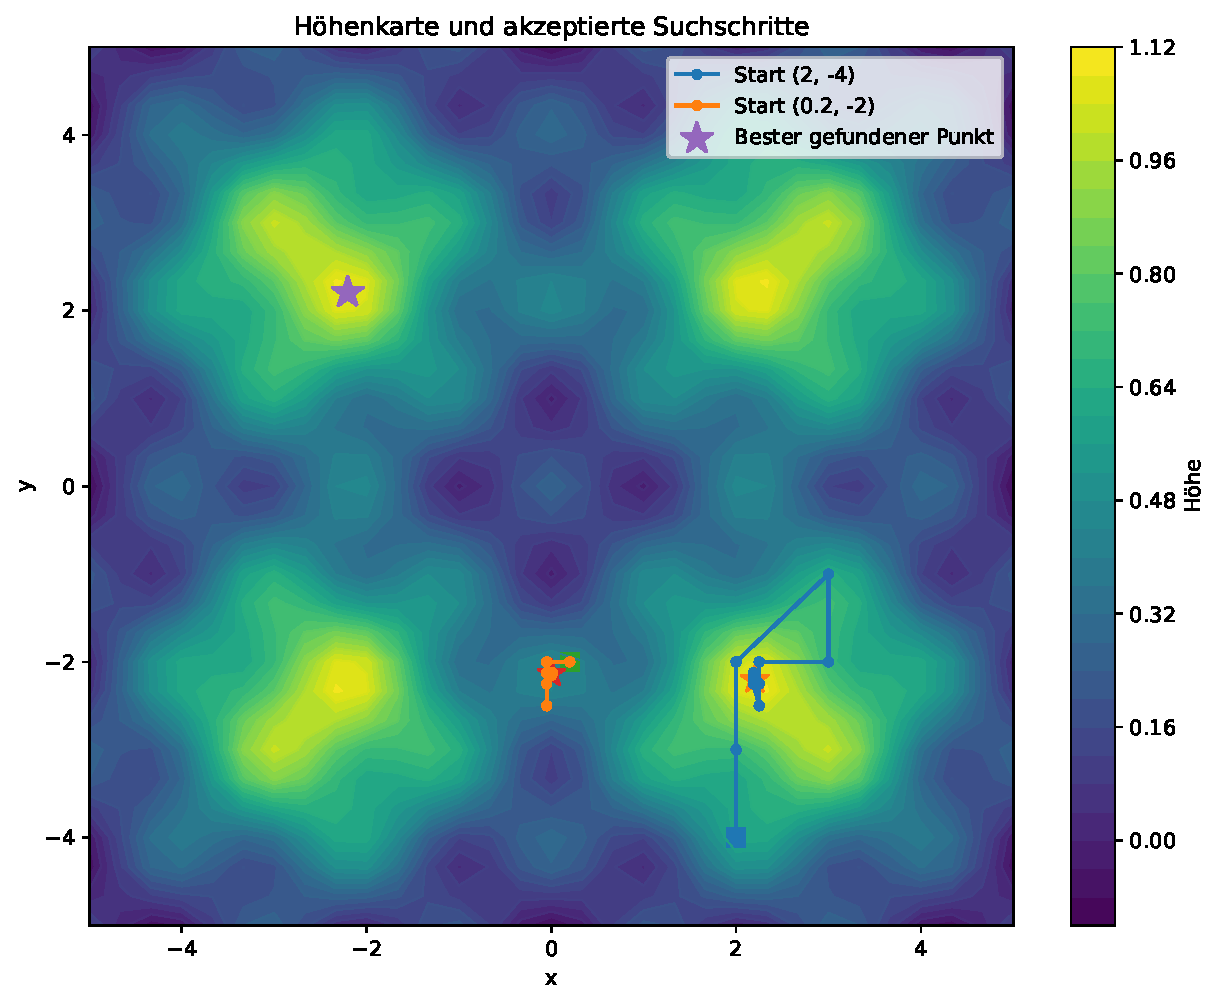
\includegraphics[width=0.8\linewidth,height=\textheight,keepaspectratio]{figures/contour_paths.pdf}

}

\caption{Konturkarte der grob ausgewerteten Höhenlandschaft mit den
akzeptierten Suchschritten der beiden vorgeschriebenen Starts. Quadrate
kennzeichnen Startpunkte und Sterne gefundene Endpunkte.}

\end{figure}%

\section{Bewertung und Fazit}\label{bewertung-und-fazit}

Die lokale Mustersuche benötigt wesentlich weniger Auswertungen als eine
entsprechend feine vollständige Gittersuche, kann aber abhängig vom
Startpunkt in einem lokalen Maximum enden. Die Kombination mit einem
groben Raster und mehreren räumlich getrennten Startpunkten reduziert
dieses Risiko.

Ein formaler Beweis globaler Optimalität ist im vorliegenden
Blackbox-Szenario ohne zusätzliche Eigenschaften der Funktion nicht
möglich. Das wiederholte Erreichen sehr ähnlicher Höhenwerte durch
mehrere Suchläufe liefert jedoch eine numerische Plausibilisierung des
gefundenen höchsten Punktes.

Die vollständigen Suchpfade, verworfenen Kandidaten, die interaktive
3D-Oberfläche und die Animation befinden sich unter:

\url{https://leobayer.github.io/Wissenschaftliche-Arbeiten/Operations_Research_Level09/}




\end{document}
